\section{Implementation}

\subsection{Pipeline Structure and Intermediate Outputs}

The implementation follows a three-stage pipeline.
Each stage produces intermediate results
that are reused by later stages.
All intermediate outputs are saved to disk
to allow modular processing and easier debugging. Table~\ref{tab:pipeline_outputs} summarizes the main intermediate outputs
produced by each stage of the pipeline.


\begin{table}[h]
    \centering
    \caption{Pipeline stages and saved intermediate outputs}
    \begin{tabular}{|l|p{5.2cm}|}
    \hline
    \textbf{Stage} & \textbf{Saved Outputs} \\
    \hline
    Preparation &
    Hand-free frame, keyboard ROI, masked keyboard image,
    white and black key coordinates (JSON),
    key overlay image \\
    \hline
    Hand analysis &
    Tracked fingertip positions,
    finger landmarks,
    per-finger press information (CSV) \\
    \hline
    Integration &
    Fingertip-to-key mapping,
    pressed keys per frame,
    final visualization video \\
    \hline
    \end{tabular}
    \label{tab:pipeline_outputs}
\end{table}


\subsection{Frame Extraction and Hand-Free Frame Selection}

Input videos are processed frame by frame.
Frames are sampled at a fixed rate.
Among the sampled frames,
a frame with minimal hand occlusion is selected manually.
This frame is used for keyboard and key detection.

\subsection{Keyboard Region Localization and Masking}

The piano keyboard region is localized
using contour-based analysis.
A bounding box is estimated
to isolate the keyboard from the background.
This bounding box defines the region of interest (ROI).

\begin{figure}[t]
    \centering
    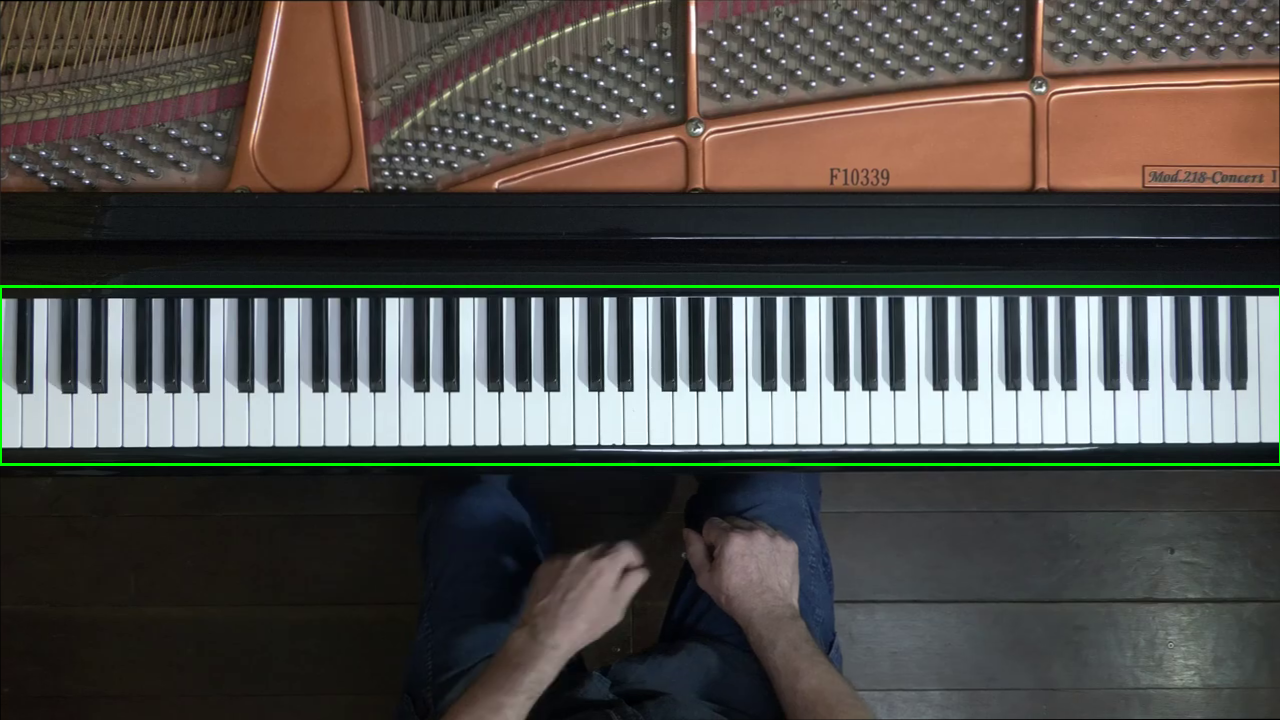
\includegraphics[width=0.85\linewidth]{figures/roi_box.png}
    \caption{Estimated keyboard region of interest (ROI) obtained from the hand-free frame.}
    \label{fig:roi}
\end{figure}

A binary mask is applied to the ROI.
Only pixels belonging to the keyboard are preserved.
Background regions are removed.
This simplifies the subsequent key detection process.

\begin{figure}[t]
    \centering
    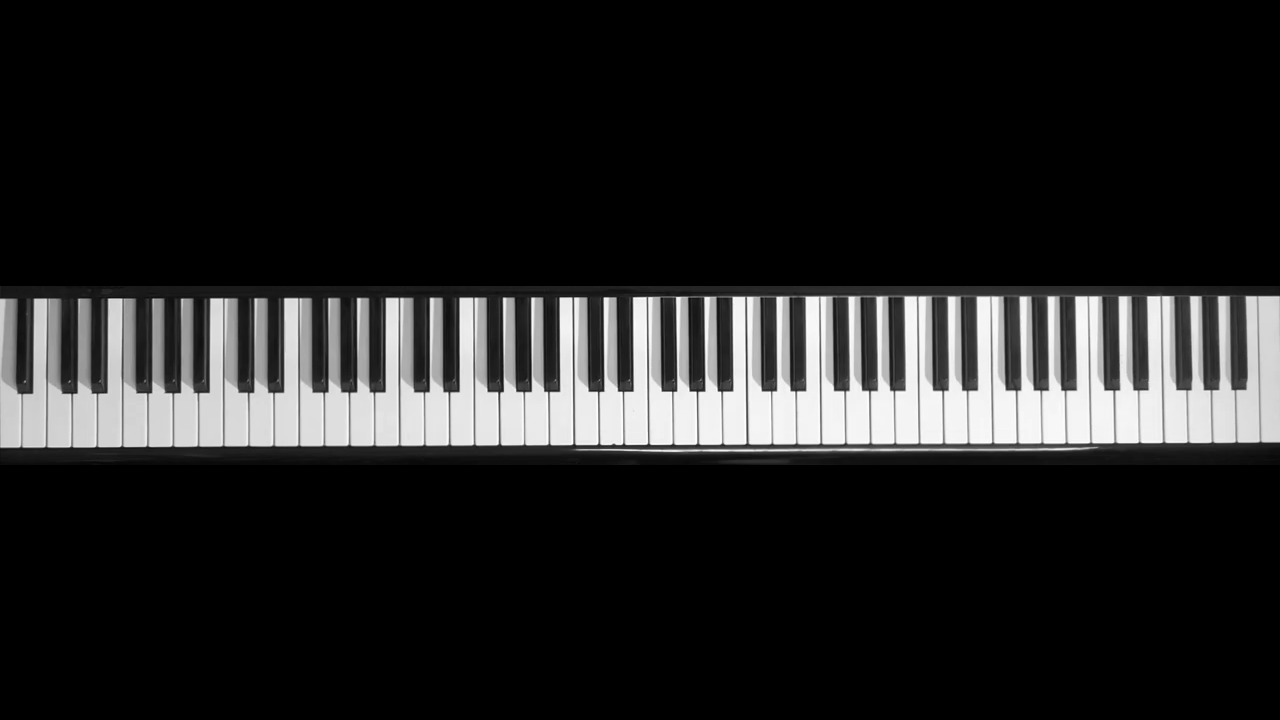
\includegraphics[width=0.85\linewidth]{figures/masked_piano.png}
    \caption{Masked keyboard image after background removal.}
    \label{fig:mask}
\end{figure}


\subsection{White and Black Key Detection}

Key detection is performed on the masked and cropped keyboard image.
White keys are detected first.
Vertical intensity transitions are analyzed
to locate borders between adjacent white keys.
The median distance between detected borders
is used to estimate the average white key width.

Using this width,
a regular grid of white key bounding boxes is generated.
The height of white keys is estimated
from the keyboard region dimensions
and kept constant across the keyboard.

Black keys are detected relative to the white key layout.
Only valid musical positions are considered.
Detection is restricted to the upper portion of the white keys,
where black keys are expected to appear.

All detected key coordinates
are initially expressed in the cropped image reference frame.
They are then mapped back to the full image reference frame
using the known ROI position and scale.
The final key locations are stored as JSON files.

\begin{figure}[t]
    \centering
    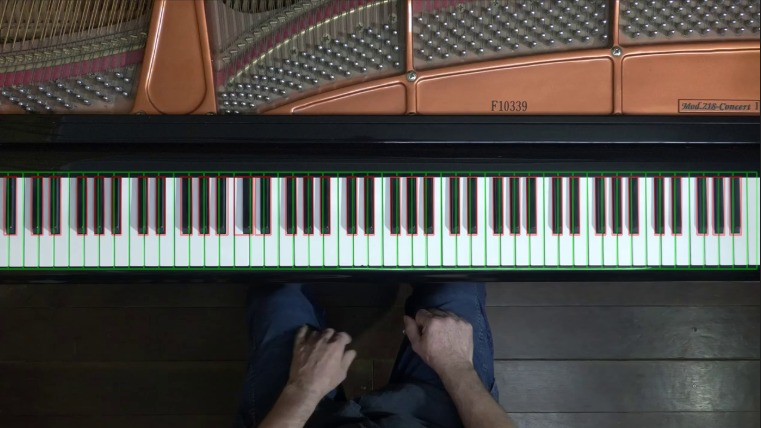
\includegraphics[width=0.85\linewidth]{figures/key_overlay.jpeg}
    \caption{Detected white and black piano keys overlaid on the full image.}
    \label{fig:keys}
\end{figure}

\subsection{Hand Motion Analysis and Press Action Detection}
\label{sec:hand_analysis}

The goal of this section is to analyse hand motion during piano performance and extract the
information required to infer key pressing events. Unlike keyboard geometry estimation,
which relies mainly on static image features, hand analysis must operate reliably under
dynamic conditions such as rapid motion, partial occlusions, and varying finger poses.
The proposed approach therefore combines deep-learning-based hand landmark detection
with geometric analysis of finger articulation and temporal filtering.

The module produces two main outputs:

\begin{itemize}
\item Fingertip coordinates for each frame
\item A binary press state for each finger over time.
\end{itemize}

\subsubsection{Fingertip Detection}
\label{subsec:fingertip_detection}

Reliable fingertip localization is a fundamental prerequisite for determining the interaction
between fingers and keys. Classical contour-based approaches based on convex hulls or
convexity defects were considered but found to be sensitive to segmentation noise and
finger overlap. For this reason, a learning-based hand landmark detection approach was adopted.

We employ MediaPipe Hands, a pretrained hand pose estimation framework capable of
predicting $21$ landmarks for each detected hand in image coordinates. The fingertips are
identified by selecting the landmark indices corresponding to the distal points of the thumb,
index, middle, ring and little fingers.

The processing pipeline for each frame consists of:

\begin{enumerate}
\item detecting the hand region
\item estimating the full set of hand landmarks
\item extracting fingertip coordinates
\item storing the results in a structured CSV representation.
\end{enumerate}

\begin{figure}[t]
\centering
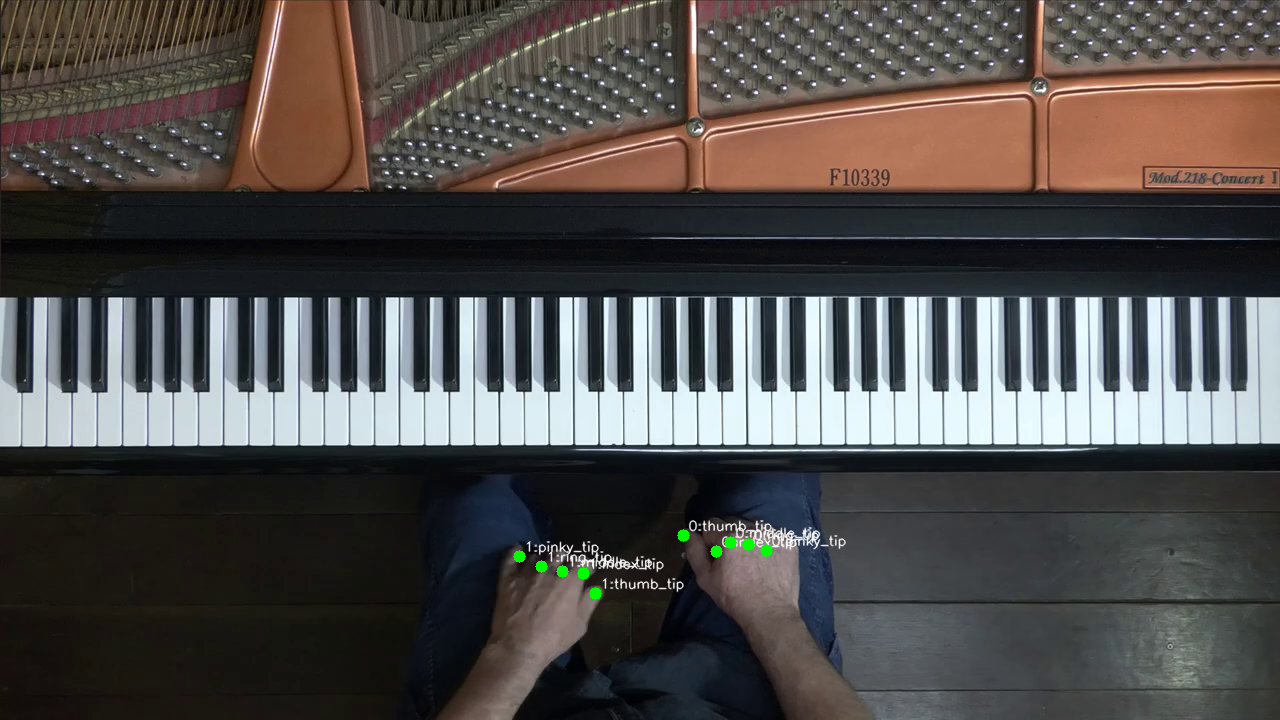
\includegraphics[width=0.85\linewidth]{figures/step2-one-frame-fingertips.png}
\caption{Example frame showing detected hand landmarks and fingertip positions obtained using MediaPipe Hands.}
\label{fig:fingertips_example}
\end{figure}

Figure~\ref{fig:fingertips_example} illustrates an example of the detected hand landmarks
and fingertip positions.

\subsubsection{Temporal Tracking and Refinement}
\label{subsec:temporal_tracking}

Since landmark detection is performed individually per frame, the output of raw detection may vary or skip due to motion blur or self-occlusion. In order to keep things stable, the fingertip paths are further refined with temporal consistency constraints. In detail:

\begin{itemize}
\item ddetection is connected between consecutive frames
\item outliers are removed
\item small detection gaps are filled with temporal filtering
\end{itemize}

This provides smooth fingertip paths, which are important for stable motion-based analysis in the following steps.

\subsubsection{Press Action Detection}
\label{subsec:press_action_detection}

The position of the fingertips is not enough to identify the press of a key as the fingers can be moved without pressing keys laterally or hovers above without applying pressure. Thus, press detection is posed as a study of finger articulation. The point to note here is that striking a piano key usually causes a typical bending of the finger. The geometric features are calculated using the complete set of hand landmarks and are measured. Inter-finger distances between pairs of joints picked. A decrease of these distances is a sign of increased finger flexion.

For each frame and for each finger:

\begin{enumerate}
\item joint-distance features are calculated
\item based on these distances, there are bending metrics
\item The state of the press is determined by the threshold-based classification
\end{enumerate}

The thresholds were chosen empirically to compromise between sensitivity to real presses and robustness. against normal hand motion.

\subsubsection{Temporal Stabilization of Press Decisions}
\label{subsec:temporal_stabilization}

Instantaneous press decisions may vary due to noise in landmark detection and/or the presence of motion artefacts. Temporal smoothing is carried out on the binary press decisions. In this step, short-term temporal consistency is ensured by:

\begin{itemize}
\item Removing single frame decisions
\item stabilizing short press intervals
\item reducing flickering between pressed and non-pressed states.
\end{itemize}

The press-state sequence now provides a stable sequence of finger activities, which will eventually be used with keyboard geometry and finger-to-key associations to determine the pressed keys.

\subsection{Key-Finger Mapping}

For each frame, fingertip positions were compared
with detected key bounding boxes.
A fingertip was assigned to a key
if it was located inside the corresponding key region.
Multiple fingertip detections were handled independently.

\subsection{Pressed-Key Detection}

Key press events were detected over time.
A key was considered pressed when a fingertip
remained inside its region across consecutive frames.
Short temporal smoothing was applied
to reduce spurious detections.
